\documentclass[12pt]{article}

\input{preamble-aufgaben}

\usetikzlibrary{positioning, arrows, shapes, automata}

% =======================================================
%\newcounter{blattnr}
\setcounter{blattnr}{12}
\newcommand{\ausgabetermin}{28.~Januar 2016}
\newcommand{\abgabetermin}{5.~Februar 2016}
%\newcommand{\punkteblatt}{13} % Blatt 1
%\newcommand{\punkteblattphysik}{13} % Blatt 1
%\newcommand{\punkteblatt}{17} % Blatt 2
%\newcommand{\punkteblattphysik}{14} % Blatt 2
%\newcommand{\punkteblatt}{18} % Blatt 3
%\newcommand{\punkteblattphysik}{18} % Blatt 3
%\newcommand{\punkteblatt}{18} % Blatt 4
%\newcommand{\punkteblattphysik}{18} % Blatt 4
%\newcommand{\punkteblatt}{18} % Blatt 5
%\newcommand{\punkteblattphysik}{18} % Blatt 5
%\newcommand{\punkteblatt}{20} % Blatt 6
%\newcommand{\punkteblattphysik}{20} % Blatt 6
%\newcommand{\punkteblatt}{20} % Blatt 7
%\newcommand{\punkteblattphysik}{0} % Blatt 7
%\newcommand{\punkteblatt}{18} % Blatt 8
%\newcommand{\punkteblattphysik}{18} % Blatt 8
%\newcommand{\punkteblatt}{17} % Blatt 9
%\newcommand{\punkteblattphysik}{17} % Blatt 9
%\newcommand{\punkteblatt}{16} % Blatt 10
%\newcommand{\punkteblattphysik}{16} % Blatt 10
%\newcommand{\punkteblatt}{19} % Blatt 11
%\newcommand{\punkteblattphysik}{19} % Blatt 11
\newcommand{\punkteblatt}{18} % Blatt 12
\newcommand{\punktetotal}{212} %
\newcommand{\punkteblattphysik}{18} % Blatt 12
\newcommand{\punktetotalphysik}{189} %
% =======================================================

\begin{document}

%\noindent
%Mit \textbf{[nicht Physik]} gekennzeichnete Aufgaben müssen von
%Studenten der Physik nicht bearbeitet werden.\\

% -----------------------------------------------------------------------------

\begin{aufgabe}[1 + 1,5 + 1,5 = 4]
  Der endliche Akzeptor $A = (Z, z_0, X, f, F)$ sei gegeben durch % $A = (\{\#0, \#1, \#2, \#3\}, \#0, \{\#a, \#b\}, f, \{\#3\})$
  \begin{center}
    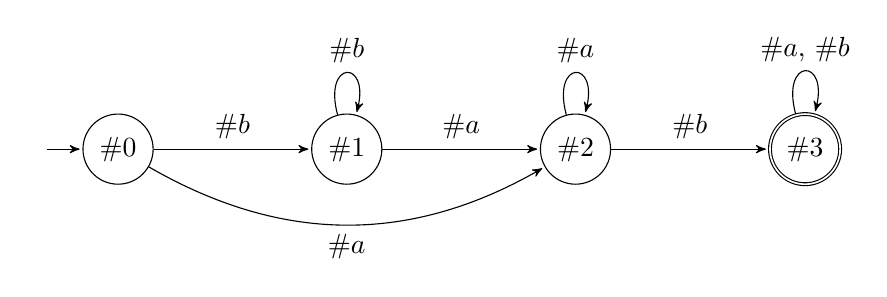
\begin{tikzpicture}[>=stealth', shorten >= 1pt, auto, node distance = 2cm, baseline=(current bounding box.north)]
      \node[initial, initial text =, state] (0) {$\#0$};
      \node[state] (1) [right = of 0]  {$\#1$};
      \node[state] (2) [right = of 1]  {$\#2$};
      \node[state, accepting] (3) [right = of 2]  {$\#3$};

      \path[->]
        (0) edge [bend right] node [below] {$\#a$} (2)
        (0) edge node {$\#b$} (1)
        (1) edge node {$\#a$} (2)
        (1) edge [loop above] node {$\#b$} ()
        (2) edge [loop above] node {$\#a$} ()
        (2) edge node {$\#b$} (3)
        (3) edge [loop above] node {$\#a$, $\#b$} ()
      ;
    \end{tikzpicture}
  \end{center}
  \begin{enumerate}
    \item Geben Sie die von $A$ akzeptierte Sprache $L(A)$, unter ausschließlicher Benutzung der formalen Sprachen $\{\#a\}$, $\{\#b\}$, sowie $\{\#a, \#b\}$, des Konkatenationsabschlusses und des Produkts formaler Sprachen, an.

          \emph{Beispiel:} $\{\#a, \#b\}^* \cdot \{\#a\} \cdot \{\#b\}$
    \item Geben Sie graphisch einen endlichen Akzeptor $B$ mit drei Zuständen an, der dieselbe formale Sprache wie $A$ akzeptiert.
    \item Geben Sie graphisch einen endlichen Akzeptor $C$ mit fünf Zuständen an, von denen zwei akzeptierend sind, der dieselbe formale Sprache wie $A$ akzeptiert.
  \end{enumerate}
\end{aufgabe}

\begin{loesung}
  \begin{enumerate}
    \item $L(A) = \{\#b\}^* \cdot \{\#a\} \cdot \{\#a\}^* \cdot \{\#b\} \cdot \{\#a, \#b\}^*$

      \begin{korrektur}
        Punktabzug bei Benutzung von Vereinigung, \usw: 
      \end{korrektur}
    \item 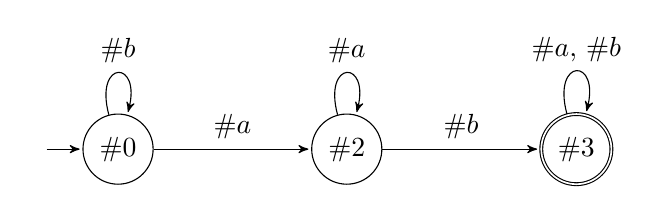
\begin{tikzpicture}[>=stealth', shorten >= 1pt, auto, node distance = 2cm, baseline=(current bounding box.north)]
            \node[initial, initial text =, state] (0) {$\#0$};
            \node[state] (2) [right = of 0]  {$\#2$};
            \node[state, accepting] (3) [right = of 2]  {$\#3$};

            \path[->]
              (0) edge node {$\#a$} (2)
              (0) edge [loop above] node {$\#b$} ()
              (2) edge [loop above] node {$\#a$} ()
              (2) edge node {$\#b$} (3)
              (3) edge [loop above] node {$\#a$, $\#b$} ()
            ;
          \end{tikzpicture}
    \item 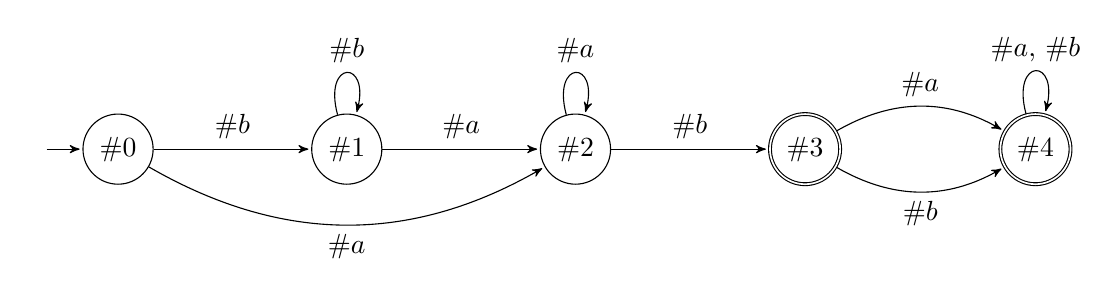
\begin{tikzpicture}[>=stealth', shorten >= 1pt, auto, node distance = 2cm, baseline=(current bounding box.north)]
            \node[initial, initial text =, state] (0) {$\#0$};
            \node[state] (1) [right = of 0]  {$\#1$};
            \node[state] (2) [right = of 1]  {$\#2$};
            \node[state, accepting] (3) [right = of 2]  {$\#3$};
            \node[state, accepting] (4) [right = of 3]  {$\#4$};

            \path[->]
              (0) edge [bend right] node [below] {$\#a$} (2)
              (0) edge node {$\#b$} (1)
              (1) edge node {$\#a$} (2)
              (1) edge [loop above] node {$\#b$} ()
              (2) edge [loop above] node {$\#a$} ()
              (2) edge node {$\#b$} (3)
              (3) edge [bend left] node [above] {$\#a$} (4)
              (3) edge [bend right] node [below] {$\#b$} (4)
              (4) edge [loop above] node {$\#a$, $\#b$} ()
            ;
          \end{tikzpicture}
  \end{enumerate}

  \begin{korrektur}
    Bei den EA: Punktabzüge für
    \begin{itemize}
    \item fehlenden Startzustand -1/3 Punkt
    \item fehlende Doppelkringel -1/3 Punkt
    \item fehlende Pfeile
      \begin{itemize}
      \item falls bei üblicher Interpretation EA richtig: -1/3
      \item falls bei üblicher Interpretation EA falsch: -2/3
      \end{itemize}
    \item Nichtdeterminismus: 
      \begin{itemize}
      \item falls bei üblicher Interpretation EA richtig: -1/3
      \item falls bei üblicher Interpretation EA falsch: -2/3
      \end{itemize}
    \item falls korrekte Wörter nicht akzeptiert oder falls nicht
      korrekte Wörter akzeptiert: jeweils -1/3 \bzw -2/3 je nachdem ob
      endlich oder unendlich viele Wörter falsch behandelt
    \item am Ende auf halbe Punkte runden
    \end{itemize}
  \end{korrektur}
\end{loesung}

% -----------------------------------------------------------------------------

\begin{aufgabe}[2 + 1 + 1 + 3 = 7]
  \begin{enumerate}
    \item Geben Sie graphisch einen endlichen Akzeptor $A$ an, der die formale Sprache $\{\#a^n \mid \exists k \in \N_0 : 5 k = n\}$ akzeptiert.
    \item Geben Sie die formale Sprache an, die der Akzeptor $B = (Z, z_0, X, f, Z \smallsetminus F)$ erkennt, wobei $A = (Z, z_0, X, f, F)$ Ihr endlicher Akzeptor aus der vorangegangenen Teilaufgabe sei.
    \item Es sei $C = (Q, q_0, Y, g, G)$ ein endlicher Akzeptor. Geben Sie, unter ausschließlicher Benutzung der formalen Sprachen $Y^*$ sowie $L(C)$, der Mengenoperationen $\cup$, $\cap$ und $\smallsetminus$, des Konkatenationsabschlusses und des Produkts formaler Sprachen, sowie eventuell runder Klammern, die formale Sprache an, die der endliche Akzeptor $D = (Q, q_0, Y, g, Q \smallsetminus G)$ akzeptiert.
    \item Geben Sie für jede nicht-negative ganze Zahl $p$ einen endlichen Akzeptor $A_p$ an, der die formale Sprache $L_p = \{\#a^{p \cdot k} \mid k \in \N_0\}$ akzeptiert.
  \end{enumerate}
\end{aufgabe}

\begin{loesung}
  \begin{enumerate}
    \item 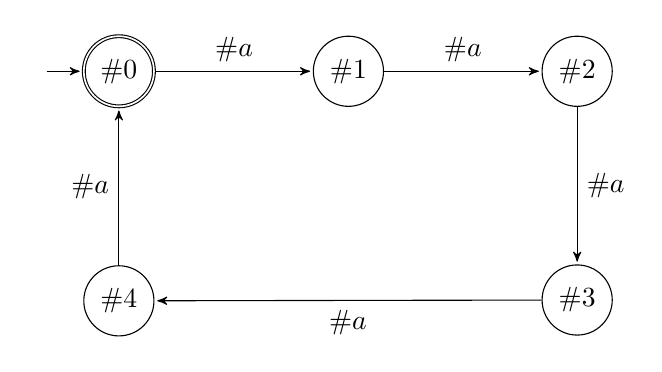
\begin{tikzpicture}[>=stealth', shorten >= 1pt, auto, node distance = 2cm, baseline=(current bounding box.north)]
            \node[initial, initial text =, state, accepting] (0) {$\#0$};
            \node[state] (1) [right = of 0]  {$\#1$};
            \node[state] (2) [right = of 1]  {$\#2$};
            \node[state] (3) [below = of 2]  {$\#3$};
            \node[state] (4) [below = of 0]  {$\#4$};

            \path[->]
              (0) edge node {$\#a$} (1)
              (1) edge node {$\#a$} (2)
              (2) edge node {$\#a$} (3)
              (3) edge node {$\#a$} (4)
              (4) edge node {$\#a$} (0)
            ;
          \end{tikzpicture}
    \item $L(B) = \{\#a^n \mid \forall k \in \N_0 : 5 k \neq n\}$
    \item $L(D) = Y^* \smallsetminus L(C)$
    \item Zunächst sei $p = 0$, also $L(A_p)=\{\eps\}$. Für $A_p = (\Z_2, 0, \{\#a\}, f, \{0\})$ mit
          \begin{align*}
            f \colon \Z_2 \times \{\#a\} &\to     \Z_2,\\
                                (z, \#a) &\mapsto 1.
          \end{align*}
          Es gilt $L(A_p) = \{\varepsilon\} = L_p$.

          Nun sei $p \in \N_+$. Weiter sei $A = (\Z_p, 0, \{\#a\}, f, \{0\})$, wobei
          \begin{align*}
            f \colon \Z_p \times \{\#a\} &\to     \Z_p,\\
                                (z, \#a) &\mapsto \begin{dcases*}
                                                    z + 1, &falls $z + 1 \in \Z_p$,\\
                                                    0,     &sonst.
                                                  \end{dcases*}
          \end{align*}
          Es gilt $L(A_p) = L_p$.

          \begin{korrektur}
            Für Fall $p=0$ ein Punkt und für Fall $p>0$ zwei Punkte.
          \end{korrektur}
  \end{enumerate}
\end{loesung}

% -----------------------------------------------------------------------------

\begin{aufgabe}[1 + 1 + 1 + 1 = 4]
  Geben Sie, unter ausschließlicher Verwendung einelementiger Mengen, den Mengenoperationen $\cup$, $\cap$, sowie $\smallsetminus$, dem Konkatenationsabschluss und dem Produkt formaler Sprachen sowie eventuell runder Klammern, die formalen Sprachen an, die die folgenden Akzeptoren akzeptieren:
  \begin{enumerate}
    \item 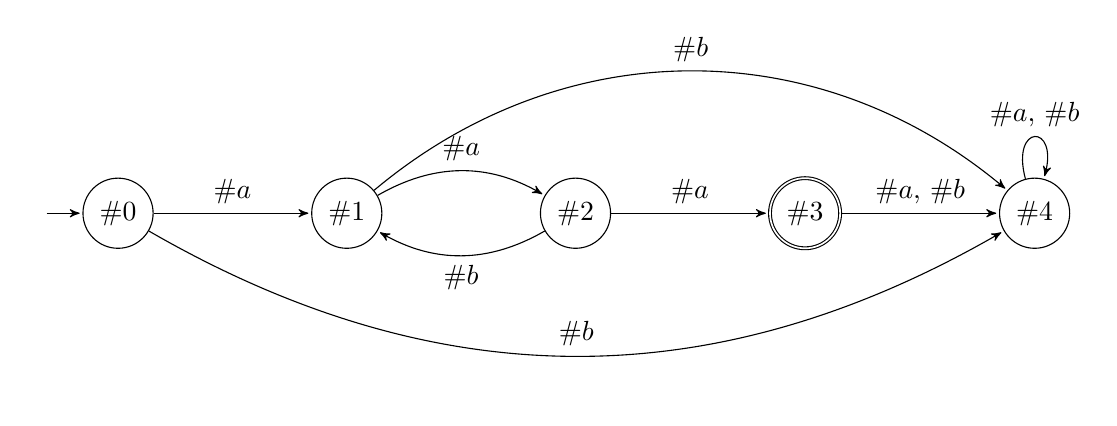
\begin{tikzpicture}[>=stealth', shorten >= 1pt, auto, node distance = 2cm, baseline=(current bounding box.north)]
            \node[initial, initial text =, state] (0) {$\#0$};
            \node[state] (1) [right = of 0]  {$\#1$};
            \node[state] (2) [right = of 1]  {$\#2$};
            \node[state, accepting] (3) [right = of 2]  {$\#3$};
            \node[state] (4) [right = of 3]  {$\#4$};

            \path[->]
              (0) edge node {$\#a$} (1)
              (0) edge [bend right = 30] node {$\#b$} (4)
              (1) edge [bend left] node {$\#a$} (2)
              (1) edge [bend left = 40] node {$\#b$} (4)
              (2) edge node {$\#a$} (3)
              (2) edge [bend left] node {$\#b$} (1)
              (3) edge node {$\#a$, $\#b$} (4)
              (4) edge [loop above] node {$\#a$, $\#b$} ()
            ;
          \end{tikzpicture}
    \item 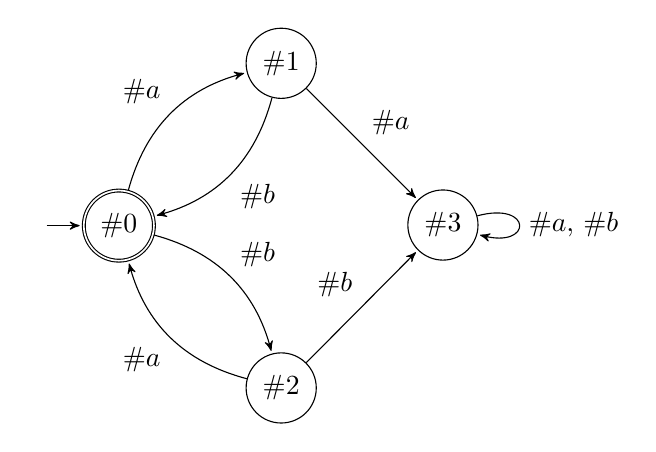
\begin{tikzpicture}[>=stealth', shorten >= 1pt, auto, node distance = 2cm, baseline=(current bounding box.north)]
            \node[initial, initial text =, state, accepting] (0) {$\#0$};
            \node[state] (1) [above right = of 0]  {$\#1$};
            \node[state] (2) [below right = of 0]  {$\#2$};
            \node[state] (3) [below right = of 1]  {$\#3$};

            \path[->]
              (0) edge [bend left] node {$\#a$} (1)
              (0) edge [bend left] node {$\#b$} (2)
              (1) edge node {$\#a$} (3)
              (1) edge [bend left] node {$\#b$} (0)
              (2) edge [bend left] node {$\#a$} (0)
              (2) edge node {$\#b$} (3)
              (3) edge [loop right] node {$\#a$, $\#b$} ()
            ;
          \end{tikzpicture}
    \item 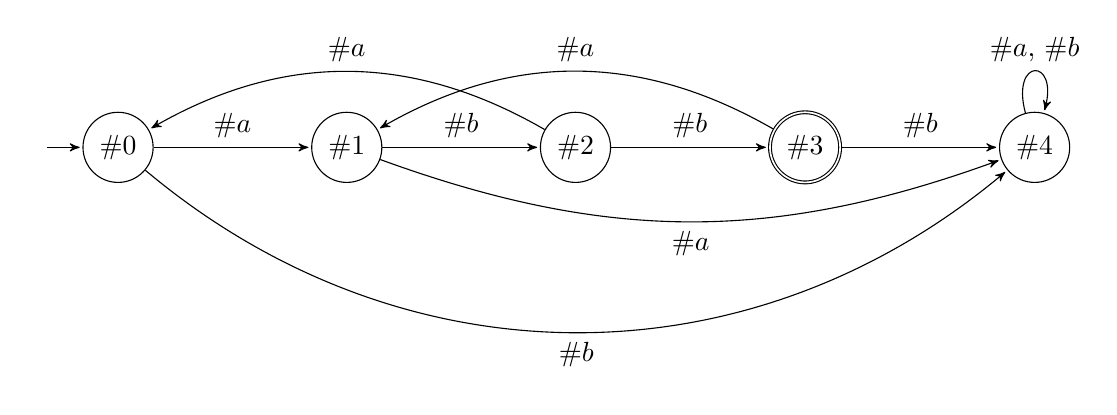
\begin{tikzpicture}[>=stealth', shorten >= 1pt, auto, node distance = 2cm, baseline=(current bounding box.north)]
            \node[initial, initial text =, state] (0) {$\#0$};
            \node[state] (1) [right = of 0]  {$\#1$};
            \node[state] (2) [right = of 1]  {$\#2$};
            \node[state, accepting] (3) [right = of 2]  {$\#3$};
            \node[state] (4) [right = of 3]  {$\#4$};

            \path[->]
              (0) edge node {$\#a$} (1)
              (0) edge [bend right = 40] node [below] {$\#b$} (4)
              (1) edge [bend right = 20] node [below] {$\#a$} (4)
              (1) edge node {$\#b$} (2)
              (2) edge [bend right] node [above] {$\#a$} (0)
              (2) edge node {$\#b$} (3)
              (3) edge [bend right] node [above] {$\#a$} (1)
              (3) edge node {$\#b$} (4)
              (4) edge [loop above] node {$\#a$, $\#b$} ()
            ;
          \end{tikzpicture}
    \item 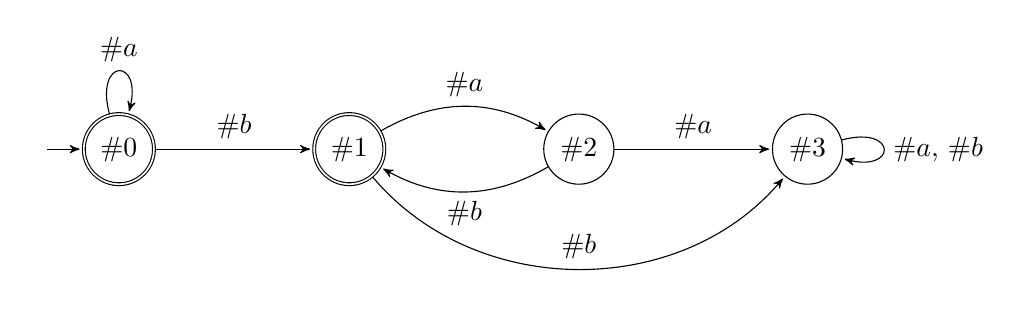
\begin{tikzpicture}[>=stealth', shorten >= 1pt, auto, node distance = 2cm, baseline=(current bounding box.north)]
            \node[initial, initial text =, state, accepting] (0) {$\#0$};
            \node[state, accepting] (1) [right = of 0]  {$\#1$};
            \node[state] (2) [right = of 1]  {$\#2$};
            \node[state] (3) [right = of 2]  {$\#3$};

            \path[->]
              (0) edge [loop above] node {$\#a$} (1)
              (0) edge node {$\#b$} (1)
              (1) edge [bend left] node {$\#a$} (2)
              (1) edge [bend right = 50] node {$\#b$} (3)
              (2) edge node {$\#a$} (3)
              (2) edge [bend left] node {$\#b$} (1)
              (3) edge [loop right] node {$\#a$, $\#b$} ()
            ;
          \end{tikzpicture}
  \end{enumerate}
\end{aufgabe}

\begin{loesung}
  \begin{enumerate}
    \item \zB $\{\#a\} \cdot \{\#{ab}\}^* \cdot \{\#{aa}\}$ oder $\{\#{aa}\} \cdot \{\#{ba}\}^* \cdot \{\#a\}$
    \item $(\{\#{ab}\} \cup \{\#{ba}\})^*$
    \item $\{\#a\} \cdot (\{\#{baa}\} \cup \{\#{bba}\})^* \cdot \{\#{bb}\}$ oder $\{\#{ab}\} \cdot (\{\#{aab}\} \cup \{\#{bab}\})^* \cdot \{\#b\}$
    \item $\{\#a\}^* \cup (\{\#a\}^* \cdot \{\#b\} \cdot \{\#{ab}\}^*)$
  \end{enumerate}
  \begin{korrektur}
    Beachte: nur einelementige Mengen erlaubt, bei Benutzung von \zB
    $\{\#{ab},\#{ba}\}$ pauschal insgesamt 1 Punkt Abzug
  \end{korrektur}
\end{loesung}

% -----------------------------------------------------------------------------

\begin{aufgabe}[3]
  Geben Sie graphisch einen endlichen Akzeptor an, der die folgende formale Sprache akzeptiert:
  \begin{equation*}
    \{\#a\} \cdot \big( (\{\#a\} \cdot \{\#b\}^* \cdot \{\#a\}) \cup (\{\#b\} \cdot \{\#a\} \cdot \{\#b\}) \big)^*
  \end{equation*}
\end{aufgabe}

\begin{loesung}
  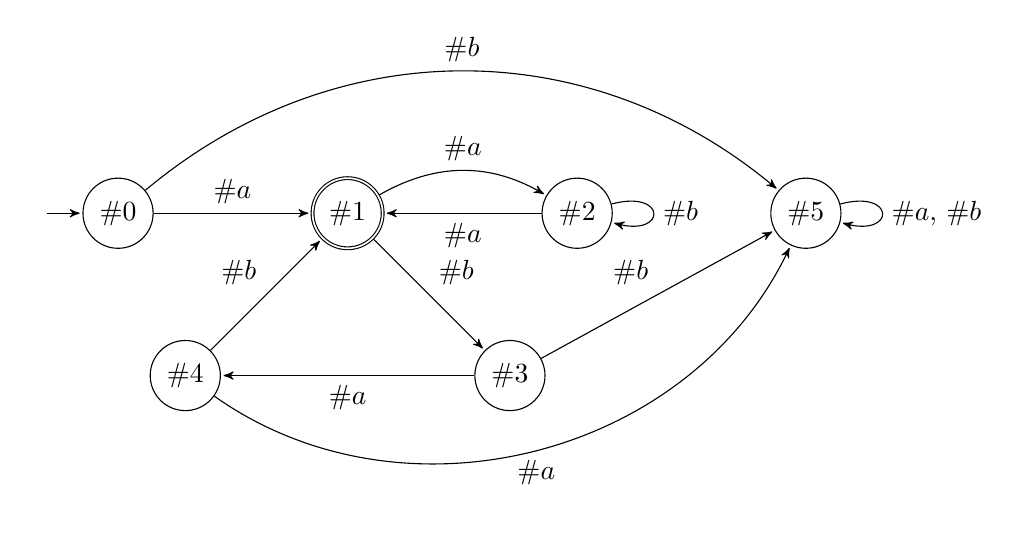
\begin{tikzpicture}[>=stealth', shorten >= 1pt, auto, node distance = 2cm, baseline=(current bounding box.north)]
    \node[initial, initial text =, state] (0) {$\#0$};
    \node[state, accepting] (1) [right = of 0]  {$\#1$};
    \node[state] (2) [right = of 1]  {$\#2$};
    \node[state] (3) [below right = of 1]  {$\#3$};
    \node[state] (4) [below left = of 1]  {$\#4$};
    \node[state] (5) [right = of 2]  {$\#5$};

    \path[->]
      (0) edge node {$\#a$} (1)
      (0) edge [bend left = 40] node {$\#b$} (5)
      (1) edge [bend left] node {$\#a$} (2)
      (1) edge node {$\#b$} (3)
      (2) edge node {$\#a$} (1)
      (2) edge [loop right] node {$\#b$} ()
      (3) edge node {$\#a$} (4)
      (3) edge node {$\#b$} (5)
      (4) edge [bend right = 50] node [below] {$\#a$} (5)
      (4) edge node {$\#b$} (1)
      (5) edge [loop right] node {$\#a$, $\#b$} ()
    ;
  \end{tikzpicture}
\end{loesung}
\begin{korrektur}
  Punktabzüge für
  \begin{itemize}
  \item fehlenden Startzustand -1/3 Punkt
  \item fehlende Doppelkringel -1/3 Punkt
  \item fehlende Pfeile
    \begin{itemize}
    \item falls bei üblicher Interpretation EA richtig: -1/3
    \item falls bei üblicher Interpretation EA falsch: -2/3
    \end{itemize}
  \item Nichtdeterminismus: 
    \begin{itemize}
    \item falls bei üblicher Interpretation EA richtig: -1/3
    \item falls bei üblicher Interpretation EA falsch: -2/3
    \end{itemize}
  \item falls korrekte Wörter nicht akzeptiert oder falls nicht
    korrekte Wörter akzeptiert: jeweils -1/3 \bzw -2/3 je nachdem ob
    endlich oder unendlich viele Wörter falsch behandelt
  \item am Ende auf halbe Punkte runden
  \end{itemize}
\end{korrektur}

% -----------------------------------------------------------------------------

\end{document}
%%%
%%% Local Variables:
%%% fill-column: 70
%%% mode: latex
%%% TeX-command-default: "XPDFLaTeX"
%%% TeX-master: "korrektur.tex"
%%% End:
